\documentclass[10pt]{beamer}
\usetheme{metropolis}
\usepackage{appendixnumberbeamer}
\usepackage{booktabs}
\usepackage[scale=2]{ccicons}
\usepackage{pgfplots}
\usepgfplotslibrary{dateplot}
\usepackage{xspace}
\newcommand{\themename}{\textbf{\textsc{metropolis}}\xspace}
%\includeonlyframes{}
%%%%%%%%%%%%%%%%%%%%%%%%%%%%%%%%%%%%%%%%%%%%%%%%%%%%%%%%%%%%%%%%%%%%%%%%%%%%%%%%
%Preambulo
%%%%%%%%%%%%%%%%%%%%%%%%%%%%%%%%%%%%%%%%%%%%%%%%%%%%%%%%%%%%%%%%%%%%%%%%%%%%%%%%
\usepackage[spanish,activeacute]{babel}
\usepackage{xcolor}
\usepackage{color}
\usepackage{colortbl}
\usepackage{amsmath}
\usepackage{amssymb}
\usepackage{graphicx}
\usepackage{latexsym}
\usepackage[T1]{fontenc}
\usepackage[utf8]{inputenc}
\usepackage{wrapfig}
\usepackage{siunitx}
\usepackage{times}
\usepackage{tikz}
\usepackage{verbatim}
\usepackage{multimedia}
\usepackage{hyperref}
\usepackage{thumbpdf}
\usepackage{pgf,pgfarrows,pgfnodes,pgfautomata,pgfheaps,pgfshade}
\usepackage{url}
\usepackage{empheq}
\usepackage{fancybox}
\usepackage{esint}
\usepackage{lipsum}
\usepackage{listings}
\usepackage{mathptmx}
\usepackage{helvet}
\usepackage{tikz}%
\usepackage{circuitikz}
\usepackage{csvsimple}
\usepackage{pgfplots}
\usepackage{multimedia}
\usepackage{media9}
\usepackage{proba}
\usepackage[absolute,overlay]{textpos}
\usepackage{bibunits}
\usepackage{tcolorbox}
%\usepackage[texcoord,grid,gridunit=mm,gridcolor=red!60,subgridcolor=green!60]%
%{eso-pic}
\pgfplotstableread[col sep = comma]{./IMAGENES/INTRODUCCION/gbm.csv}\mydata
\usepackage[makeroom]{cancel}
\usepackage{epstopdf}
\epstopdfsetup{outdir=./}
\title{Modelado con Ecuaciones Diferenciales 
    Estoc\'asticas via Perturbaci\'on de Par\'ametros}
\subtitle{y una Invitaci\'on a la soluci\'on num\'erica de EDEs}
\date{\today}
\author{Sa\'ul D\'iaz Infante Velasco}
\institute{CONACYT-Universidad de Sonora}
\titlegraphic{%
\hfill\includegraphics[height=1.0cm]{./figures/logo_unach.jpg}
}
\metroset{block=fill}
%%%%%%%%%%%%%%%%%%%%%%%%%%%%%%%%%%%%%%%%%%%%%%%%%%%%%%%%%%%%%%%%%%%%%%%%%%%%%%%%
\def\Q#1#2{\frac{\partial #1}{\partial #2}}
\usetikzlibrary{arrows,shapes}
%%%%%%%%%%%%%%%%%%%%%%%%%%%%%%%%%%%%%%%%%%%%%%%%%%%%%%%%%%%%%%%%%%%%%%%%%%%%%%%%
%------------------------------------Theorems 
\theoremstyle{plain} % default
\newtheorem{Teorema}{Teorema}
\newtheorem{Ejemplo}{Ejemplo}
\theoremstyle{definition}
\newtheorem{Definicion}{Definici\'on}
\newtheorem{Corolario}{Corolario}
\newtheorem{Proposicion}{Proposici\'on}
\newtheorem{Prueba}{Prueba}
\theoremstyle{definition}
\newtheorem{definicion}{Definici\'on}
\newtheorem{lema}{Lema}
%-----------------------------ExtrasDeTercerPresentacion
%--------------------------------Fancyboxes-------------------------------------
\definecolor{myblue}{rgb}{.8, .8, 1}
\definecolor{shadecolor}{cmyk}{0,0,0.41,0}
\newcommand*\mybluebox[1]{%
	\colorbox{myblue}{\hspace{1em}#1\hspace{1em}}
}
\newcommand*\myyellowbox[1]{%
	\colorbox{darkyellow}{\hspace{1em}#1\hspace{1em}}
}
%--------------------------------------------------------------------------
\definecolor{shadecolor}{cmyk}{0,0,0.41,0}
\definecolor{light-blue}{cmyk}{0.25,0,0,0}
\newsavebox{\mysaveboxM} % M for math
\newsavebox{\mysaveboxT} % T for text
\newcommand*\Garybox[2][Example]{%
	\sbox{\mysaveboxM}{#2}%
		\sbox{\mysaveboxT}{\fcolorbox{black}{light-blue}{#1}}%
			\sbox{\mysaveboxM}{%
	\parbox[b][\ht\mysaveboxM+.5\ht\mysaveboxT+.5\dp\mysaveboxT][b]{%
		\wd\mysaveboxM}{#2}%
	}%
	\sbox{\mysaveboxM}{%
		\fcolorbox{black}{shadecolor}{%
		\makebox[\linewidth-10em]{\usebox{\mysaveboxM}}%
		}%
	}%
	\usebox{\mysaveboxM}%
	\makebox[0pt][r]{%
		\makebox[\wd\mysaveboxM][c]{%
			\raisebox{\ht\mysaveboxM-0.5\ht\mysaveboxT
			+0.5\dp\mysaveboxT-0.5\fboxrule}{\usebox{\mysaveboxT}}%
		}%
	}%
}
\newcommand\Fontvi{\fontsize{7}{7.2}\selectfont}
%%%%%%%%%%%%%%%%%%%%%%%%%%%%%%%%%%%%%%%%%%%%
\definecolor{kugreen}{RGB}{50,93,61}
\definecolor{kugreenlys}{RGB}{132,158,139}
\definecolor{kugreenlyslys}{RGB}{173,190,177}
\definecolor{kugreenlyslyslys}{RGB}{214,223,216}
\definecolor{greenArea}{RGB}{124,252,124}
\definecolor{hellmagenta}{rgb}{1,0.75,0.9}
\definecolor{hellcyan}{rgb}{0.75,1,0.9}
\definecolor{hellgelb}{rgb}{1,1,0.8}
\definecolor{colKeys}{rgb}{0,0,1}
\definecolor{colIdentifier}{rgb}{0,0,0}
\definecolor{colComments}{rgb}{1,0,0}
\definecolor{colString}{rgb}{0,0.5,0}
\definecolor{darkyellow}{rgb}{1,0.9,0}
\setbeamercovered{transparent}
\lstset{%
    language=[AlLaTeX]TEX,%
    float=hbp,%
    basicstyle=\ttfamily\small, %\usepackage{cir}
    identifierstyle=\color{colIdentifier}, %
    keywordstyle=\color{colKeys}, %
    stringstyle=\color{colString}, %
    commentstyle=\color{colComments}, %
    columns=flexible, %
    tabsize=3, %
    frame=single, %
    extendedchars=true, %
    showspaces=false, %
    showstringspaces=false, %
    numbers=left, %
    numberstyle=\tiny, %
    breaklines=true, %
    backgroundcolor=\color{hellgelb}, %
    breakautoindent=true, %
    captionpos=b,%
    xleftmargin=18pt,%
    xrightmargin=\fboxsep%
}
\pgfplotsset{
    left segments/.code={\pgfmathsetmacro\leftsegments{#1}},
    left segments=3,
    left/.style args={#1:#2}{
        ybar interval,
        domain=#1:#2,
        samples=\leftsegments+1,
        x filter/.code=\pgfmathparse{\pgfmathresult}
       }
}
\DeclareMathOperator{\sign}{sgn}
\newcommand{\innerprod}[2]{\left\langle#1, #2\right\rangle}
\newcommand\bound{10} % bound number of points on each side of N
\newcommand\labelnum[3][]{
	\begin{scope}[font=\footnotesize,x=.3cm,#1]
	  \foreach \mypt in {0,#2,...,\bound}{
	    \draw(\mypt,0)circle[radius=2pt];
	    \draw(-\mypt,0)circle[radius=2pt];
	  }
	  \draw(-\bound-5,0)--(\bound+5,0) node[pos=0, left]{$t$};
	  \node(start)[at={(-\bound-4,0)},label=below:{$t_0=0$}]{$[$};
	  \node(end)[at={(\bound+4,0)},label=below:{$T=Nh$}]{$]$};
	  \node[%
		  at={($(start)!.319!(end)$)},
		  label=below:{
			   $\underbrace{}_{h}$
			}%
			]{\vphantom{$[$}};
	  \node[at={($(start)!.57!(end)$)},label=below:{$t_{n+1}$}]{\vphantom{$[$}};
	  \filldraw(0,0)circle[radius=2pt];
	  \node[at={(-\bound-2,0)},above]{$\cdots$};
	  \node[at={(\bound+2,0)},above]{$\cdots$};
	  \node[at={(0,0)},above=5pt]{#3};
	\end{scope}
}
\tcbuselibrary{skins,breakable}

\defaultbibliography{CharlaBib}
\defaultbibliographystyle{abbrv}
\begin{document}
    \maketitle
    \section*{Introducci\'on}
        \begin{frame}
  \frametitle{Por que EDEs?}
    \begin{empheq}[box={\Garybox[En ocaciones]}]{align*}
        EDO+ruido=Mejor \text{ } modelo
    \end{empheq}
    \begin{overlayarea}{\textwidth}{.8\textheight}
        \begin{columns}
            \column{.55\textwidth}
            \only<2-3>{
                \begin{exampleblock}{Crecimiento de Poblaciones}
                    $$
                        \frac{dN}{dt}=a(t)N(t) \qquad N_0=N(0)=cte.
                    $$
                \end{exampleblock}
            }
            \only<4-6>{
            \begin{exampleblock}{Circuitos Eléctricos}
                \begin{align*}
                   &L\cdot Q''(t)+
                    R\cdot Q'(t)+
                    \frac{1}{C}\cdot Q(t)
                        =F(t)
                    \\
                   &Q(0)=Q_0\\
                   &Q'(0)=I_0
                \end{align*}
            \end{exampleblock}
        }
        \column{.58\textwidth}
        \only<3>{
            \begin{empheq}[box=\shadowbox*]{equation*}
                a(t)=r(t)+"ruido"
            \end{empheq}
        }
        \only<5-6>{
            %\includegraphics[width=\textwidth]{./images/CircuitRLC.png}
            \begin{circuitikz}[american voltages]
                \draw (0,0)
                to[sV,v=$F(t)$] (0,2) % The voltage source
                to[R=$R$, i^>=$i(t)$] (2,2) % The resistor
                to[L=$L$] (4,2)
                to[C=$C$] (4,0)--(0,0) ;
            \end{circuitikz}
        }
        \only<6>{
            \begin{empheq}[box=\shadowbox*]{equation*}
                F(t)=G(t)+"ruido"
            \end{empheq}
        }
        \end{columns}
    \end{overlayarea}
\end{frame}
%%%%%%%%%%%%%%%%%%%%%%%%%%%%%%%%%%%%%%%%%%%%%%%%%%%%%%%%%%%%%%%%%%%%%%%%%%%%%%%%%%
\begin{frame}
    \frametitle{Para fijar ideas}
    \begin{empheq}[box={\Garybox[Ejemplo]}]{align*}
        dN(t) = aN(t)dt
    \end{empheq}
    \begin{overlayarea}{\textwidth}{.3\textheight}
        \begin{columns}
            \column{.5\textwidth}
                \only<2->{
                    \begin{block}{Perturba sobre $[t, t+dt)$}
                        \only<3->{
                            $$
                              a dt
                              \rightsquigarrow
                              a dt + \sigma dB(t)
                            $$
                        }
                    \end{block}
               }
            \column{.5\textwidth}
        \only<4->{
            \begin{exampleblock}{obten una EDE}
              $$
               dN(t) = aN(t)dt + \sigma N(t) dB(t)
              $$
            \end{exampleblock}
        }
        \end{columns}
    \end{overlayarea}
    \begin{overlayarea}{\textwidth}{.7\textheight}
        \centering
            \resizebox{0.45\textwidth}{!}{%
            \only<5>{
                \begin{tikzpicture}
                    \begin{axis}[%
                     line width=1.0pt,
                     mark size=1.0pt
                     ]%
                         \addplot[color=blue]%
                         table [%
                           x index = {0},
                           y index = {1} %
                       ]{\mydata};
                       \addplot[domain=0:5, samples=100]{1.5*exp(x)};
                    \end{axis}
                \end{tikzpicture}
         }
        }
    \end{overlayarea}
\end{frame}
%   %\section{}
%%%%%%%%%%%%%%%%%%%%%%%%%%%%%%%%%%%%%%%%%%%%%%%%%%%%%%%%%%%%%%%%%%%%%%%%%%%%%%%%%
    \begin{frame}{Esquema de Charla}
        \setbeamertemplate{section in toc}[sections numbered]
        \tableofcontents[hideallsubsections]
    \end{frame}
    \section{Construcción de Métodos Numéricos}
        \subsection{EDEs en sentido de It^o}
            \begin{frame}
  \frametitle{Notación}
  \begin{empheq}[box={\Garybox[
		\hyperlink{thm:ExistenciaUnicidadEDE}{EDE}]}
  ]{align*}
    \only<1-3>{
    dx(t)&= 
 			\underbrace{f(x(t),t)dt}_{\text{deriva}} 
 			+
 			\underbrace{g(x(t),t) dB(t)}_{\text{difusión}},\\
	  }
	  \only<2-3>{
				x_0 &= x(0), \quad
				t\in[0,T].\\
			}
 	  \only<4>{
 	  x(t) &= x_0 + \int_0^t f(x(s),s)ds
		  +
		  \int_0^t g(x(s),s)dB(s)
 	  }
  \end{empheq}
	\hypertarget<4>{frm:notacion}
	\only<3->{
		\begin{align*}
			&f:\R ^d 
				\times [0,T] \to \R^d,
			\qquad
			g:\R^d 
				\times [0,T] \to \R^{d\times m} \\
			&B(t)=\left(B_1(t),\dots,B_m(t)\right)^T,
			\quad
			\left(
				\Omega, \calF, \{\calF_t\}_{t\geq 0}, \P
			\right)
		\end{align*}
	}
\end{frame}

             \begin{frame}
   \frametitle{Idea general de la construcción}
  \begin{empheq}[box={\Garybox[EDE]}]{align*}
 	  x(t) &= x_0 + \int_0^t f(x(s),s)ds
		  +
		  \int_0^t g(x(s),s)dB(s)
	\end{empheq}
	\only<2->{
		\centering
		\begin{tikzpicture}
		  \labelnum[yshift=-2cm]{2}{Stencil}
		\end{tikzpicture}
	}
 	\only<3>{
		\begin{equation*}
			x(t_{n+1}) = 
			x(t_{n}) 
			+
			\int_{t_{n}}^{t_{n+1}} f(x(s),s)ds
		  +
		  \int_{t_{n}}^{t_{n+1}} g(x(s),s)dB(s)
		\end{equation*}
	}
	\only<4-6>{
		\begin{equation*}
			x(t_{n+1}) = 
			x(t_{n}) 
			+
			\underbrace{
				\int_{t_{n}}^{t_{n+1}} f(x(s),s)ds
		  }_{%
				  \textcolor<5-6>{red}{%
					  \approx \text{det}%
					 }
				}
		  +
		  \underbrace{
			  \int_{t_{n}}^{t_{n+1}} g(x(s),s)dB(s)
			}_{%
					\textcolor<6>{red}{%
						\hyperlink{frm:integracion}{\approx}
						%\approx
						}
				}
		\end{equation*}
	}
	\hypertarget<6>{frm:incremento_bm}{}
	\only<7->{
		\begin{equation*}
			x(t_{n+1}) = 
			x(t_{n}) 
			+
			\underbrace{
				\int_{t_{n}}^{t_{n+1}} f(x(s),s)ds
		  }_{%
				  \textcolor{red}{%
					  \approx 
					   f(x_n) h
					 }
				}
		  +
		  \underbrace{
			  \int_{t_{n}}^{t_{n+1}} g(x(s),s)dB(s)
			}_{
				\substack{
					\approx 
					g(x_n) \Delta B_n \\
					\Delta B_n = B_{t_{n+1}}-B_{t_n}
				}
			}
		\end{equation*}
	}
	\only<7>{
		\begin{textblock*}{.25\textwidth}(4.5cm,3.0cm)
			\begin{exampleblock}{}
				% left hand sums
				\centering
				\begin{tikzpicture}[scale=0.3,%
				/pgf/declare function={f=-15*(x-5)+(x-5)^3+50;}]
					\begin{axis}[
					        xmin=0,xmax=8,ymin=0,ymax=80,
					    domain=0:10,
					    samples=100,
					    axis lines=middle
					]
					\addplot [thick, red] {f};
					\addplot [
					    black!80,fill=green,opacity=.3,
					    left segments=7,
					    left=1:6
					] {f};
					\end{axis}
				\end{tikzpicture}
			\end{exampleblock}
		\end{textblock*}
	}
 	\only<8>{
		\begin{align*}
				X_0 &=x_0, \qquad X_n  \approx x(t_n),
				\qquad 
				n=1 \dots, N-1
				\\
				X_{n+1} &= X_n + f(X_n) h + g(X_n) \Delta B_n, 
		 \end{align*}
	}
 	\only<9>{
 		\begin{align*}
 			X_0 &=x_0, \qquad X_n  \approx x(t_n),
 			\qquad 
 			n=1 \dots, N-1
 			\\
 			X_{n+1} &= X_n + f(X_n) h + g(X_n) 
 			\textcolor{blue}{%
 				\underbrace{\Delta B_n}_{%
 					\approx
 				}%
 			}%
 	 \end{align*}
 	}
\end{frame}

        \subsection{Aproximaci\'on de Movimiento Browninano}
            \input{./AproximacionDeMB/random_walks.tex}
        \subsection{Construcci\'on del Euler-Mayurama}
        \section{Aproximaci\'on Fuerte vs. D\'ebil}
            \begin{frame}
  \frametitle{Debil vs Fuerte}
  \begin{empheq}[box={\Garybox[dada]}]{align*}
 		dx(t)
			&=f(x(t))dt + g(x(t)) dB(t), 
 		\\
			x(0) &= x_0, \quad t\in[0,T]
 	\end{empheq}
  \begin{overlayarea}{\textwidth}{.7\textheight}
    \begin{columns}
      \column{.58\textwidth}
        \begin{block}{Debil}
          $$
						X_{n+1} = X_n + f(X_n) h 
							+ g(X_n) 
							\underbrace{\Delta B_n}_{%
								\substack{
									\approx \sqrt{h} \varepsilon_n\\
									\probX{\varepsilon_n=\pm 1}=1/2
								}
							}
					$$
        \end{block}
        %%%%%%%%%%%%%%%%%%%%%%%%%%%%%%%%
        \column{.58\textwidth}
          \begin{exampleblock}{Fuerte}
          $$
						X_{n+1} = X_n + f(X_n) h 
							+ g(X_n) 
							\underbrace{\Delta B_n}_{%
								\substack{
									\approx \sqrt{h} \epsilon_n\\
									\epsilon_n \sim N(0,1)
								}
							}
					$$
          \end{exampleblock}
    \end{columns}
  \end{overlayarea}
\end{frame}
    \section{Ejemplo: Reconstrucción de masa osea}
        % %%%%%%%%%%%%%%%%%%%%%%%%%%%%%%%%%%%%%%%%%%%%%%%%%%
\begin{frame}{Proceso de Remodelación en BMU}
	\begin{tikzpicture}[remember picture,overlay]
	  \node[anchor=south west, inner sep=0pt] at (current page.south west) {%
    \movie[%
	    height = \paperheight,%
	    width = \paperwidth,%
	    poster,%
			showcontrols]{}{./Video/oc-ob.mp4}%
      };
  \end{tikzpicture}
\end{frame}

        %%%%%%%%%%%%%%%%%%%%%%%%%%%%%%%%%%%%%%%%%%%%%%%%%%%%%%%%%%%%%%%%5
\begin{frame}
	\frametitle{Fases de remodelación}
		\only<1-2>{%
			\includegraphics[width=\textwidth,keepaspectratio]{%
			./IMAGES/Komarova/boneRemodeling.png%
			}
		}
		\only<3-4>{%
			\includegraphics[width=.9\textwidth,keepaspectratio]{%
			./IMAGES/Komarova/boneRemodeling.png%
			}
		}

 		\only<1-2>{
			\begin{textblock*}{105mm}(10mm, 70mm)
				\begin{block}{Fases del proceso de remodelación}
						\begin{bibunit}[apalike]
						\nocite{Raggatt2010}
						\putbib
					\end{bibunit}
				\end{block}
			\end{textblock*}
 		}
\end{frame}

        \begin{frame}{}
	\frametitle{El Modelo de Komarova}
 	\only<1->{
		\begin{textblock*}{40mm}(10mm, 20mm)
			\begin{align*}
 			\frac{du}{dt} &=
 				u^{\kappa_1}
				\left(
					\alpha_1 v^{\gamma_1} - \beta_1
				\right)
				\\
			\frac{dv}{dt} &=
				v^{\kappa_2}
				\left(
					\alpha_2 u^{\gamma_2} - \beta_2
				\right)
			\\
			\only<3->{
					\frac{dz}{dt} &=
				-
				k_1 \max\{u - \widetilde{u}, 0\}
				\\
				&
				+
				k_1 \max\{v - \widetilde{v}, 0\}
			}
				\end{align*}
		\end{textblock*}
 	}
	\only<4>{% modelote
		\begin{textblock*}{.9\textwidth}(10mm, 5mm)
			\begin{exampleblock}{Descripción}
				\includegraphics[width=.98\textwidth, keepaspectratio]%
				{./IMAGES/Komarova/komarovaModelDescripcion.png}
			\end{exampleblock}
		\end{textblock*}	
	}
	\only<5>{% modelote
		\begin{textblock*}{.9\textwidth}(10mm, 5mm)
			\begin{exampleblock}{Descripción}
				\includegraphics[width=.98\textwidth, keepaspectratio]%
				{./IMAGES/Komarova/komarovaModelDescripcionb.png}
			\end{exampleblock}
		\end{textblock*}	
	}
	%
	\only<6>
	{
		\begin{textblock*}{.5\textwidth}(60mm, 20mm)
			\includegraphics[width=\textwidth, keepaspectratio]%
			{./IMAGES/Komarova/komarovaModel1.png}
		\end{textblock*}
	}
	\only<2-4>{
		\begin{textblock*}{100mm}(10mm, 63mm)
			\begin{bibunit}[alpha]
				\nocite{Komarova2003}
				%\biblio{CharlaBib.bib}
				\putbib
		  \end{bibunit}
  \end{textblock*}
	}
\end{frame}

        \begin{frame}{}
	\frametitle{Simplificación}
 	\only<1->{
		\begin{textblock*}{40mm}(10mm, 20mm)
			\begin{align*}
				\only<1>{
					\frac{du}{dt} &=
						u^{\kappa_1}
						\left(
							\alpha_1 v^{\gamma_1} - \beta_1
						\right)
						\\
					\frac{dv}{dt} &=
						v^{\kappa_2}
						\left(
							\alpha_2 u^{\gamma_2} - \beta_2
						\right)
					\\
 				}
				\only<2>{
					\frac{du}{dt} &=
					u^{
						\xcancel{\kappa_1}
					}
					\left(
						\alpha_1 v^{\gamma_1} - \beta_1
					\right)
					\\
				\frac{dv}{dt} &=
					v^{
						\xcancel{\kappa_2}
					}
					\left(
						\alpha_2 u^{\gamma_2} - \beta_2
					\right)
				\\
				}
				\only<3->{
					\frac{du}{dt} &=
					u
					\left(
						\alpha_1 v^{\gamma_1} - \beta_1
					\right)
					\\
				\frac{dv}{dt} &=
					v
					\left(
						\alpha_2 u^{\gamma_2} - \beta_2
					\right)
				\\
				} 			
				\only<5->{
						\frac{dz}{dt} &=
					-
					k_1 \max\{u - \widetilde{u}, 0\}
					\\
					&
					+
					k_1 \max\{v - \widetilde{v}, 0\}
				}
				\end{align*}
		\end{textblock*}
 	}
	\only<4>{% modelote
		\begin{textblock*}{1.2\textwidth}(0mm, 0mm)
			\includegraphics[width=\textwidth, keepaspectratio]%
			{./IMAGES/Komarova/silviaModelDescripcion.png}
		\end{textblock*}	
	}
%
	\only<6>
	{
		\begin{textblock*}{.5\textwidth}(60mm, 15mm)
			\includegraphics[width=\textwidth, keepaspectratio]%
			{./IMAGES/Komarova/silviaModel1.png}
		\end{textblock*}
	}
	\only<7>
	{
		\begin{textblock*}{.5\textwidth}(60mm, 15mm)
			\includegraphics[width=\textwidth, keepaspectratio]%
			{./IMAGES/Komarova/silviaModel2.png}
		\end{textblock*}
	}
	
	
	\only<3->{
		\begin{textblock*}{100mm}(10mm, 65mm)
			\begin{bibunit}[alpha]
				\nocite{Jerez2015a}
				\putbib
		  \end{bibunit}
  \end{textblock*}
	}
\end{frame}

        \begin{frame}
	\frametitle{¿Por qué incorporar incertidumbre a un modelo?}
	\begin{textblock*}{37mm}(3mm, 10mm)
		\begin{block}{Efectos Ambientales}
			\begin{itemize}
				\item \textcolor<2-3>{orange}{Extinción}
				\item \textcolor<4>{orange}{Epidemias}
			\end{itemize}
		\end{block}
	\end{textblock*}
	\begin{textblock*}{75mm}(45mm, 10mm)
		\begin{alertblock}{%
				\only<2>{%
					Ruido ambiental suprime extinción%
				}%
				\only<3>{%
					Color (correlación) induce extinción
				}%
				\only<4>{%
					$\mathcal{R}_0$: endémico g.a.e $\to$ osc. per 
					%$\mathcal{R}_0$ (determinista)
				}%
		}%Block titles
			\only<2>{
				\begin{bibunit}[apalike]
					\nocite{Mao2002}
					\putbib
			  \end{bibunit}
			}
			\only<3>{
				\begin{bibunit}[apalike]
					\nocite{Ripa1996}
					\putbib
			  \end{bibunit}
			}
			\only<4>{
				\begin{bibunit}[apalike]
					\nocite{Allen2013}
					\putbib
			  \end{bibunit}
			}
		 \end{alertblock}
	\end{textblock*}
\end{frame}
        \begin{frame}
	\frametitle{Alternativas}
	\begin{textblock*}{37mm}(3mm, 10mm)
		\begin{block}{Efectos Ambientales}
			\begin{itemize}
				\item Extinción
				\item Epidemias
			\end{itemize}
		\end{block}
	\end{textblock*}
%%%%%%%%%%%%%%%%%%%%%%%%%%%%%%%%%%%%%%%%%%%%%%%%%%%%%%%%%%%%%%%%%%%%%%%%%%%%%%%
	\begin{textblock*}{37mm}(3mm, 35mm)
		\begin{block}{En biología}
			\begin{itemize}
				\item<2> \textcolor<2>{orange}{CTMCs}
				\item<3-4,6>\textcolor<3-4,6>{orange}{
					\textbf<6>{%
						Perturbación de parámetros
					}
				}
				\item<5> \textcolor<5>{orange}{Procesos reversibles en media}
			\end{itemize}
		\end{block}
	\end{textblock*}
%%%%%%%
	\begin{textblock*}{75mm}(45mm, 35mm)
		\begin{alertblock}{%
				\only<2>{%
					$\mathbf{MC}+\mathbf{ME}$ $\to$ $SDE$%
				}%
				\only<3,6>{%
					$\varphi dt \rightsquigarrow \varphi dt+ \sigma dB_t$%
				}%
				\only<4>{%
					$\varphi dt \rightsquigarrow \varphi dt+F(x)dB_t$%
				}%
				\only<5>{%
					$d \varphi_t = (\varphi_e -\varphi_t)dt + \sigma_\varphi dBt$ %
				}%
		}%Block titles
			\only<2>{
				\begin{bibunit}[apalike]
					\nocite{Allen2017}
					\putbib
			  \end{bibunit}
			}
			\only<3>{
				\begin{bibunit}[apalike]
					\nocite{Gray2011}
					\putbib
			  \end{bibunit}
			}
			\only<4>{
				\begin{bibunit}[apalike]
					\nocite{Schurz2015}
					\putbib
			  \end{bibunit}
			}
			\only<5>{
				\begin{bibunit}[apalike]
					\nocite{Allen2016}
					\putbib
			  \end{bibunit}
			}
		 \end{alertblock}
	\end{textblock*}
\end{frame}


        \input{./Perturbacion/perturbacion.tex}
        \subsection{Propiedades de la solución}
            \input{./PropiedadesSolucion/positividad.tex}
        \subsection{Resultados numéricos}
        %%%%%%%%%%%%%%%%%%%%%%%%%%%%%%%%%%%%%%%%%%%%%%%%%%
%\begin{frame}[plain]	
%	\begin{columns}
%		\column[t]{60mm}
%			%\begin{tikzpicture}[remember picture,overlay]
%% 			\node[anchor=south west, inner sep=0pt] at (%
%% 				current page.south west) {%
% 			\movie[%
%				height = \textwidth,,%
%				width = 1.1\textwidth,%
%				poster,%
%				%keepaspectratio,
%				showcontrols]{}{./Video/StoPLBRM.mp4}%
%% 				};
%% 		\end{tikzpicture}
%		%\end{textblock*}
%		\column[t]{50 mm}
%		%\begin{textblock*}{.5\textwidth}(65mm, 20mm)
%				\includegraphics[width=.9\textwidth, keepaspectratio]{%
%					./IMAGES/ComparacionDeModelos/pfSilvia.png}
%		%\end{textblock*}	
%	\end{columns}	
%\end{frame}
%%%%%%%%%%%%%%%%%%%%%%%%%%%%%%%%%%%%%%%%%%%%%%%%%%%%%%%%%%%%%%%
\begin{frame}[plain]{Comparación de Fases}
	\includegraphics[width=\textwidth,keepaspectratio]{%
		./IMAGES/LongShortTime/ComparacionDeFase.png}
\end{frame}
%%%%%%%%%%%%%%%%%%%%%%%%%%%%%%%%%%%%%%%%%%%%%%%%%%%%%%%%%%%%%%%
\begin{frame}[plain]{PF tiempo corto (7 años) vs timpo largo (80-90 años)} 
	\includegraphics[width=\textwidth,keepaspectratio]{%
		%./IMAGES/LongShortTime/PhasePotrait3d(a).png
		./IMAGES/LongShortTime/ComparacionDePlanosFase.png%
		}
\end{frame}
%%%%%%%%%%%%%%%%%%%%%%%%%%%%%%%%%%%%%%%%%%%%%%%%%%%%%%%%%%%%%%%
\begin{frame}[plain]{Oscilaciones en torno a $\xi_i$}
	\includegraphics[width=\textwidth,keepaspectratio]{%
		%./IMAGES/LongShortTime/PhasePotrait3d(b).png
		./IMAGES/LongShortTime/OscilacionesXi1Xi2.png%
		}
\end{frame}
%%%%%%%%%%%%%%%%%%%%%%%%%%%%%%%%%%%%%%%%%%%%%%%%%%%%%%%%%%%%%%%
\begin{frame}[plain]{Trayectoria larga y  masa osea}
	\includegraphics[width=\textwidth,keepaspectratio]{%
		./IMAGES/LongShortTime/longPahtBoneMass.png}
\end{frame}
%%%%%%%%%%%%%%%%%%%%%%%%%%%%%%%%%%%%%%%%%%%%%%%%%%%%%%%%%%%%%%%
\begin{frame}[plain]{Momentos a tiempo corto (13 años)}
	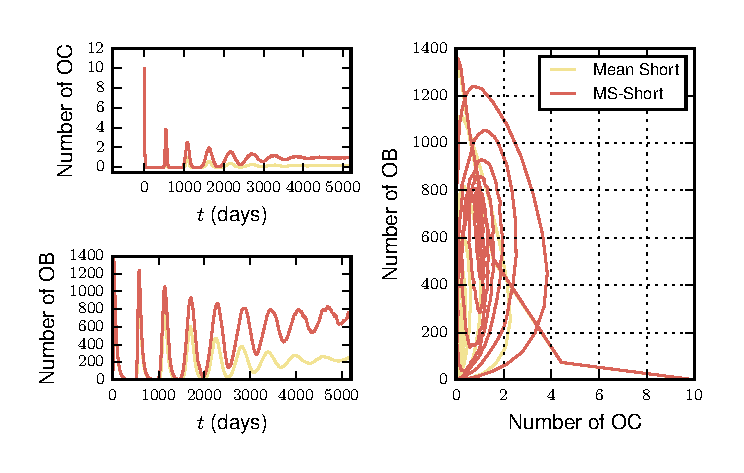
\includegraphics[width=\textwidth,keepaspectratio]{%
		./IMAGES/LongShortTime/shortTimeMoments.png}
\end{frame}
%%%%%%%%%%%%%%%%%%%%%%%%%%%%%%%%%%%%%%%%%%%%%%%%%%%%%%%%%%%%%%%
\begin{frame}[plain]{Momentos a tiempo largo}
	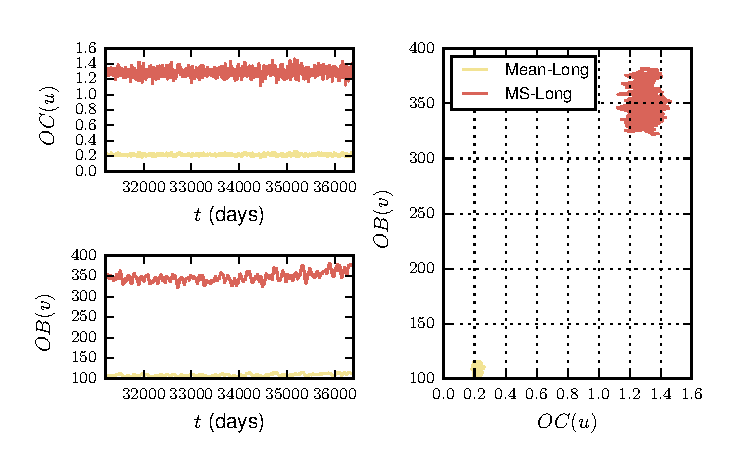
\includegraphics[width=\textwidth,keepaspectratio]{%
		./IMAGES/LongShortTime/longTimeMoments.png}
\end{frame}
%%%%%%%%%%%%%%%%%%%%%%%%%%%%%%%%%%%%%%%%%%%%%%%%%%%%%%%%%%%%%%%

    \section{Comentarios Finales}
        \begin{frame}[plain]
    \only<1-3>{
    \begin{textblock*}{100mm}(10mm, 40mm)
        \begin{block}{}
            \begin{bibunit}[alpha]
                \nocite{Jerez2017}
                %\biblio{CharlaBib.bib}
                \putbib
            \end{bibunit}
        \end{block}
    \end{textblock*}
    }
     \only<2>{
        \begin{textblock*}{60mm}(40mm, 20mm)
            \Huge Gracias!!!
        \end{textblock*}
    }
\end{frame}
\begin{frame}
    \href{https://github.com/SaulDiazInfante/Beamer-xxx-semana-unison-2020-AppliedMathematicsWorkshop-.git}{Git-Hub}
    \flushright
    \qrcode{https://github.com/SaulDiazInfante/Beamer-xxx-semana-unison-2020-AppliedMathematicsWorkshop-.git}
\end{frame}
    \appendix
        \begin{frame}{}
	\frametitle{Funci\'on caracter\'istica}
	\hypertarget{dfn:FuncionCaracteristica}{}
	\begin{block}{Definici\'on (Funci\'on caracter\'istica)}
			Sea $X$ 
			v. a., entonces,
			$$
				\phi_{X}(t)= \EX{ e^{i t X}}, \qquad t \in \R,
			$$
		es la función característica de $X$.
	\end{block}
	\uncover<2>{
	\begin{block}{Teorema de continuidad}
		Sea 
		$
			\{ X_{n} \}_{n=1}^{\infty}   \quad v.a.
		$, entonces
		$$ 
			X_{n} \xrightarrow{\mathcal{D}} X \Leftrightarrow 
			\phi_{X_{n}}(t) 
			\to \phi_{X}(t) .
		$$
	\end{block}
	}
	\hyperlink{cns:Limite}{\beamerreturnbutton{Const}}
\end{frame}
%%%%%%%%%%%%%%%%%%%%%%%%%%%%%%soluciones-------------------
 \begin{frame}
   \frametitle{Integral Estocástica}
   \hypertarget{frm:integracion}{}
   \begin{empheq}[box={\Garybox[Integral]}]{align*}
 			& \int_{0}^T f(\cdot) d 
 			\only<1-2>{
				(\cdot)
 			}
 			\only<3->{
				B(\cdot)
 			} 
 			\\ 
				\only<2>{
					&
					f: [0, T] \to \R 
				} 
				\only<3->{
					&
					f: [0,T] \times \Omega \to \R
				}
  	\end{empheq}
   \begin{overlayarea}{\textwidth}{.7\textheight}
			\only<2->{
				\hyperlink{frm:incremento_bm}{Determinista:}
				$$
					\int_{0}^T f(\cdot) d(\cdot)
					\approx
					\sum_{j=0}^{N-1}
						f(t_j) (t_{j+1} - t_{j})
				$$
			}
			\begin{columns}
				\column[t]{.5\textwidth}
					\only<3->{
						\begin{block}{It\^o}
							$$
								\approx
								\sum_{j=0}^{N-1}
									f(t_{j})
									(B_{t_{j+1}} - B_{t_j})
							$$
						\end{block}
				}
				%%%%%%%%%%%%%%%%%%%%%%%%%%%%%%%%%
				\column[t]{.5\textwidth}
				\only<4>{	
					\begin{exampleblock}{Stratonovich}
 						$$
							\approx
 							\sum_{j=0}^{N-1}
 								f
  							\left(
									\frac{t_{j} + t_{j+1}}{2}
  							\right)
 								(B_{t_{j+1}} - B_{t_j})
 						$$
					\end{exampleblock}
				}
     \end{columns}
   \end{overlayarea}
\end{frame}
%%%%%%%%%%%%%%%%%%%%%%%%%%%%%%%%%%%%%%%%%%%%%%%%%%%%%%%%%%%%%%%%%%%%%%%%%%%%%%%
%\begin{bibunit}[apalike]
\begin{frame}
  \frametitle{Existencia y unicidad de soluciones fuertes para EDEs}
	\hypertarget{thm:ExistenciaUnicidadEDE}{}  
	%\vspace{-.50cm} 
	%\vspace{-.23cm}  
	\begin{block}{%
		Sea $dX_{t}=f(t,X_{t})dt+f(t,X_{t})dB_{t}$ 
		en el sentido de It\^{o}, t.q.
		}
		\begin{enumerate}[(EU1)]
		  \item (Medibles):
				$f,g$ son \textcolor{cyan}{$\mathcal{L}^{2}-$medibles} en
				$(t,x)\in[t_{0},T] \times \mathbb{R}^d$.
			\item (\only<2-4>{\textcolor{orange}{Local }}Lipschitz): 
				\only<1>{$\exists K>0$}  
				\only<2-4>{$\exists \textcolor{orange}{K_n}>0$}
				t.q. 
				
				$
				 \forall t\in[t_{0},T], 
				$
				$
					\forall x,y\in \mathbb{R}^d
				$
				\only<2-4>{t.q. \textcolor{orange}{$|x-y|\leq n$}}
				\only<1>{
					\begin{align*}
						\textcolor{red}{|f(t,x)-f(t,y)|}
								\textcolor{red}{\leq K|x-y|}, 
						\quad	
						\textcolor{red}{|g(t,x)-g(t,y)|}
								\textcolor{red}{\leq K|x-y|}
					\end{align*}
				}
				\only<2-4>{
					\begin{align*}
						\textcolor{red}{|f(t,x)-f(t,y)|}
								\textcolor{orange}{\leq K_n|x-y|},
							\quad	
						\textcolor{red}{|g(t,x)-g(t,y)|}
							\textcolor{orange}{\leq K_n|x-y|}
					\end{align*}
				}
			\item 
				\only<1-2>{	
					(De crecimiento lineal):
				}
				\only<3-4>{
					(\textcolor{orange}{Monotonia})
				}
				$
					\exists K>0$, 
				t.q. 
				$
					\forall t\in[t_{0},T],
					\quad  \forall x\in\mathbb{R}^d
				$
				\only<1-2>{
					\begin{align*}
						\textcolor{red}{|f(t,x)|^{2}}
							\textcolor{red}{\leq K^{2}(1+|x|^{2})},
						\quad
						\textcolor{red}{|g(t,x)|^{2}}
							\textcolor{red}{\leq K^{2}(1+|x|^{2})}
					\end{align*}
				}
				\only<3-4>{
					$$
						\textcolor{orange}{
							\innerprod{x}{f(t,x)} 
						+ 
							|g(x)|^2 \leq K(1+|x|^2)
						}
					$$
				}
		  \item (Condición inicial): 
			  $X_{t_{0}}$ es
			  $\mathcal{F}_{t_{0}}-$medible con 
			  $
				  \EX{|X_{t_{0}}|}<\infty
				$.
		\end{enumerate}
		Entonces, \colorbox{darkyellow}{$ \exists ! X_{t}$} en
		$[t_{0},T]$ con  \colorbox{darkyellow}{
			$\displaystyle
				 \sup_{t_{0}\leq t\leq T}
				 \mathbb{E}(|X_{t}|^{2})<\infty$.
				 }
	\end{block}
	\hyperlink{frm:notacion}{\beamerreturnbutton{Construccion}}
\end{frame}
% %\end{bibunit}
%----------------------------Promedio 
%Steklov---------------------------------------------
% %\begin{bibunit}[apalike]
% \begin{frame}
%   \frametitle{Promedio de Steklov}
% 	\hypertarget{dfn:Steklov}{}    
%   \begin{overlayarea}{\textwidth}{.5\textwidth}
%       \begin{block}{Promedio de Steklov} %\cite{matus2005exact}}
% 	  \begin{align*}	  		
% 	  		F(X_t)\approx \varphi(X_n,X_{n+1})=&
% 		        \left(
% 		        \frac{1}{X_{n+1}-X_{n}}
% 		        \int_{X_n}^{X_{n+1}} \frac{du}{F(u)}
% 		        \right)^{-1}\\
% 		      	t_n\leq & t \leq t_{n+1},\\
% 		      	X_n=&X_{t_n}, \quad t_n=nh.	 
% 	  \end{align*}
%     \end{block}
%   \end{overlayarea}   
% \hyperlink{ex:EDEMult}{\beamerreturnbutton{Ej:EDEMult}}\\
% \hyperlink{Idea}{\beamerreturnbutton{idea}}  
% %\biblio{BibliografiaTesis}
% \end{frame}
% %\end{bibunit}
% %%%%%%%%%%%%%%%%%%%%%%%%%%%%%%%%%%%%%%%%%%%%%%
\begin{frame}
  \frametitle{Lema de Gronwall}
	\hypertarget{lem:Gronwall}{}
     \begin{lema}[de Gronwall]
		Sean $\alpha,\beta:[t_0,T]\to\mathbb{R}$ funciones integrables t.q.
		$$
			0\leq \alpha(t)\leq \beta(t) +L \int_{t_0}^{t}\alpha(s)ds 
			\qquad t\in[t_0,T].
		$$
		Entonces 
		$$
			\alpha(t)\leq \beta(t)+L\int_{t_0}^{t} e^{L(t-s)}\beta(s)ds
		$$
		\end{lema}
	\hyperlink{prb:Consistencia2}{\beamerreturnbutton{Prueba}}\\
	\hyperlink{Idea}{\beamerreturnbutton{idea}}
	%\biblio{BibliografiaTesis}
\end{frame}
% %%%%%%%%%%%%%%%%%%%%%%%%%%%%%%%%%%%%%%%%%%%%%
\begin{frame}
  \frametitle{Desigualdad de Lyapunovl}
	\hypertarget{thm:DesLyapunov}{}    
	Sea $X$ una v.a integrable y $0<q\leq p$ entonces    
    \begin{block}{Sea $X$ una v.a integrable y $0<q\leq p$ entonces}
		$$    	
    		\mathbb{E}\left(\left|X\right|^{q}\right)\leq\mathbb{E}\left(\left|X\right|^{p}\right)^{\frac{q}{p}}
		$$    
    \end{block}
	\hyperlink{prb:Consistencia3}{\beamerreturnbutton{Prueba}}
%\hyperlink{Idea}{\beamerreturnbutton{idea}}  
%\biblio{BibliografiaTesis}
\end{frame}
%%%%%%%%%%%%%%%%%%%%%%%%%%%%%%%%%%%%%%%%%%%%%
\begin{frame}
  \frametitle{Isometría de It\^{o}}
	\hypertarget{thm:Isometria}{}    	
	\begin{block}{Propiedades Integral de It\^{o}}
		\begin{enumerate}		
		\item
			$\displaystyle		
				\mathbb{E}
				\left[
					\int_0^T g(r)dB_r
				\right]=0
			$
		\item(Isometr\'ia)
			$\displaystyle		
				\mathbb{E}
				\left[
					\left(
						\int_0^T g(r)dB_r					
					\right)^2		
				\right]=
				\int_0^T g^2(r)d	r		
			$
		\end{enumerate}	
	\end{block}	
	\hyperlink{prb:ConsistenciaISO}{\beamerreturnbutton{Prueba}}  
%\biblio{BibliografiaTesis}
\end{frame}
%%%%%%%%%%%%%%%%%%%%%%%%%%%%%%%%%%%%%%%%%%%%%%%%%%%%%%%%%%%%%%%%%%%%%%%%%%%%%%
\begin{frame}
%[label=MatrixFunctions,noframenumbering]
	\hypertarget{MatrixFunctions}
	\frametitle{Apendice A}
	\scalebox{0.85}{\parbox{1.0\linewidth}{
		\begin{align*}	
			A^{(1)}(h,u)&:=
			\begin{pmatrix}
				e^{ha_1(u)} & 
\multicolumn{2}{c}{\text{\kern0.5em\smash{\raisebox{-1ex}{\huge 0}}}} \\
				&\ddots\\
				\multicolumn{2}{c}{\text{\kern-0.5em\smash{\raisebox{0.95ex}{\huge 
0}}}} 
				& e^{ha_d(u)}
			\end{pmatrix},
			\\
		%	
			A^{(2)}(h,u)&:=
			\begin{pmatrix}
				\left(
					\displaystyle
					\frac{e^{ha_1(u)} - 1}{a_1(u)}
				\right)\1{E_1^c}	& 
				\multicolumn{2}{c}{\text{\kern0.5em\smash{\raisebox{-1ex}{\huge 0}}}}\\
				& \ddots&\\
				\multicolumn{2}{c}{\text{\kern0.5em\smash{\raisebox{-1ex}{\huge 0}}}}&
				\left(
					\displaystyle
					\frac{e^{ha_d(u)} - 1}{a_d(u)}
				\right)\1{E_d^c}% + h \1{E_i} 
			\end{pmatrix}
			+h
			\begin{pmatrix}
				\1{E_1} & 
\multicolumn{2}{c}{\text{\kern0.5em\smash{\raisebox{-1ex}{\huge 0}}}}\\
				&\ddots &\\
				\multicolumn{2}{c}{\text{\kern0.5em\smash{\raisebox{-1ex}{\huge 0}}}} &
				\1{E_d}
			\end{pmatrix},\\	
			E_j&:=\{x \in \R^d: a_j(x)=0\} , \qquad 
			b(u):= 
			\left(
				b_1(u^{(-1)}), \dots , b_d(u^{(-d)})
			\right)^T.		
		\end{align*}
		}
	}
	\\
	\hyperlink{tcb:mipropuesta}{\beamerreturnbutton{LS}}
\end{frame}
%%%%%%%%%%%%%%%%%%%%%%%%%%%%%%%%%%%%%%%%%%%%%%%%%%%%%%%%%%%%%%%%%%%%%%%%%%%%%%%%
%%%%%%%%%%%%%%%%%%
%\begin{frame}[label=ZerosConditions, noframenumbering]
%	\frametitle{Apendice B: Resultato para ceros no aislados}    
%	\begin{columns}
%		\column{.6\textwidth}
%			\begin{Teorema}[L'h\^{o}pital Multivariable] 
%				\begin{itemize}
%					\item 
%						$\mathcal{N}$ vecindad en $\R^2$ de $\mathbf{p}$ donde
%						$f:\mathcal{N}\to \R$,  
%						$g:\mathcal{N}\to \R$ diferenciables son cero. 
%					\item
%						$
%							C=\{x \in \mathcal{N}: f(x)=g(x)=0 \},
%						$				
%					\item
%						Supón $C$ suave, que pasa por $\mathbf{p}$.
%					\item
%					 $\exists \ \mathbf{v}$ no tangente a $C$ en $\mathbf{p}$
%						t.q  $D_{\mathbf{v}}g$ en la dirección $\mathbf{v}$ es no nula en
%						$\mathcal{N}$.
%					\item
%						$\mathbf{p}$ es punto limite de $\mathcal{N}\setminus C$. 
%			\end{itemize}
%	    Entonces
%				$
%					\displaystyle
%					\lim_{(x,y)\to \mathbf{p}}
%					\frac{f(x,y)}{g(x,y)} =
%					\lim_{
%						\substack{
%							(x,y)\to \mathbf{p}\\ 
%							(x,y)\in \mathcal{N} \setminus C
%						}
%					}
%					\frac{D_{\mathbf{v}} f }{D_{\mathbf{v}} g},
%				$
%				siempre que exista el limite.
%			\end{Teorema}
%			\column{.4\textwidth}
%				\includegraphics[width=\linewidth]{Imagenes/Apendice/LawlorThm.png}
%				\\
%				\hyperlink{Construccion<6>}{\beamerreturnbutton{Hip\'otesis}}
%				\begin{bibunit}[alpha]
%					\nocite{Lawlor2012}
%					\biblio{PhdThesisBib.bib}
%				\end{bibunit}
%	\end{columns}
%\end{frame}
%%%%%%%%%%%%%%%%%%%%%%%%%%%%%%%%%%%%%%%%%%%%%%%%%%%%%%%%%%%%%%%%%%%%%%%%%%%%%%%%
%%%%%%%%%%%%%%%%
\begin{frame}[noframenumbering]
	\frametitle{Apendice B: Resultado para ceros aislados}    
	\begin{columns}
		\column{.4\textwidth}
		\begin{definicion}[DD respecto a $p$]
			 $u,\mathbf{p}\in \R^2$,  $\alpha$ angulo positivo respecto a eje-$x$ 
			segmento $\overline{u \mathbf{p}}$.	 
			\begin{align*}
				f_{\alpha}(u) &= 
				\frac{ \innerprod{q-u}{\nabla f(u)}}{|u-q|}			
			\end{align*}
			 \emph{derivada direccional respecto $\mathbf{p}$ en $u$}.
		\end{definicion}
		\begin{definicion}[Star-like set]
			$S\subset \R^2$ es \emph{star-like} respecto $\mathbf{p}$,  $\forall \ s 
\in S$ 
			el segmento abierto	$\overline{s \mathbf{p}}$  esta en $S$.
		\end{definicion}

		\column{.6\textwidth}
		%\includegraphics[width=\linewidth]{Imagenes/Apendice/LawlorThm.png}
		\begin{Teorema}
			\begin{itemize}
				\item 
					$\mathbf{p}\in \R^2$, $S\subset \R^2$ star-like respecto $\mathbf{p}$ 
en el dominio de $f$,$g$.
				\item
					En $S$, $f,g$ diferenciables , $g_{\alpha}(s)\neq 0$, 	
				\item 
					$f(\mathbf{p})=g(\mathbf{p})=0$,
					\quad
					$
						\displaystyle
						\lim_{x \to \mathbf{p}}
						\frac{f_{\alpha}(x)}{g_{\alpha}(x)} = L,	
					$
			\end{itemize}
			Entonces
				$ 
					\displaystyle
					\lim_{x \to \mathbf{p}}
					\frac{f(x)}{g(x)} = L.
				$
		\end{Teorema}
		\begin{bibunit}[alpha]
			\nocite{FineAIandKass1966}
			\putbib
		\end{bibunit}
	\end{columns}
\end{frame}
%%%%%%%%%%%%%%%%%%%%%%%%%%%%%%%%%%%%%%%%%%%%%%%%%%%%%%%%%%%%%%%%%%%%%%%%%%%%%%
\begin{frame}[noframenumbering]
	\frametitle{Apéndice B: Condiciones para ceros de $a_j(\cdot)$}    
		\hypertarget{ZerosConditions}{}
		\textcolor{orange}{
			 $E_j:=\{x\in \R^{d}: a_j(x)=0\}$
		} satisface alguno de los puntos:
		\begin{enumerate}[(i)]
			\item
				 $p \in E_j$ es un cero no aislado de  $a_j(\cdot)$ y:
			\begin{itemize}
				\item  
					\textcolor{cyan}{
					$
						D:=\{u: e^{ha_j(u)}-1=a_j(u)= 0\},
					$ 
				}
				es una curva suave que pasa por $p$. 
				\item
				El vector canónico $e_j$ es no tangente a $D$.
				\item
					Para cada $p \in E_j$, existe una bola $B_r(p)$ t.q.
				$$
					a_j\neq 0, \qquad
					\frac{\partial a_j(u)}{\partial u^{(j)}} \neq 0 ,\qquad 
					\forall u \in D
					\setminus B_r(p).
				$$
			\end{itemize}	
			\item
				 $p \in E_j$ es un cero aislado de $a_j(\cdot)$ y:
			\begin{itemize}
				\item
					Para cada $q\in E_j$,  $p$ no es punto limite de
					$E_{\alpha}:=\{x \in \R^d: (a_j)_\alpha(x)=0\}$.
				\item
					Para cada $p \in E_j$ existe  $B_r(p)$, t.q.
					la derivada direccional respecto a $p$ satiface
				$$
				(a_j)_\alpha(x) \neq 0, \qquad \forall x\in B_r(p).
				$$
			\end{itemize}
		\end{enumerate}
\hyperlink{frm:condiciones_zeros}{\beamerreturnbutton{LSHyp}}
\end{frame}

\end{document}
